\SACCMD{beginframe}
\label{cmd:beginframe}

\SACTitle{概要}
关闭两次绘图之间的自动刷新框架的操作

\SACTitle{语法}
BeginFrame [PRINT [pname]]

\SACTitle{输入}
\begin{itemize}
\item PRINT pname: 当在BEGINFRAME中使用PRINT时,SAC将把图形打印到名为pname的打印机,如果pname没有指定则打印到默认的打印机
\end{itemize}

\SACTitle{其他形式}
BEGFR也是被允许的形式

\SACTitle{说明}
刷新框架操作主要是指清楚当前绘图显示的画面。通常SAC会在每个新的绘图之前(PLOT, PLOT1等)执行刷新操作,所谓自动刷新框架操作相当于每次绘图使用将原来的绘图擦除,在空白的纸张上绘制新图,以保证图不会重叠在一起。当使用BEGINFRAME命令时SAC停止执行自动刷新框架操作,当执行ENDFRAME命令时恢复自动刷新框架。因而在这两个命令之间执行的所有绘图都将输出到同一个框架中。

通过使用XVPORT、YVPORT修改不同绘图的视口(即图形占框架的位置),改变不同的绘图选项,读取不同的数据文件,这样就可以很容易生成一个一张图上有多个图形的绘图。具体细节参见下面的例子。注意你必须执行ENDFRAME结束这种模式,恢复自动刷新框架功能。

\SACTitle{例子}
下面的例子给出了beginframe使用的方法以及效果,你需要一个名为FILE1的SAC文件:
\begin{SACCode}
SAC> fg seis
SAC> beginframe          //关闭自动刷新框架
SAC> xvport .1 .9        //定义视口
SAC> yvport .7 .9
SAC> title 'SEISMIC TRACE'
SAC> fileid off
SAC> qdp off
SAC> p
SAC> fft wmean           //做FFT
SAC> xvport .1 .45       //第二个视口
SAC> yvport .15 .55
SAC> title 'Amplitude Response-linlog'
SAC> ylim 1e-5 1
SAC> psp am linlog       //绘制振幅谱
SAC> xvport .55 .9       //第三个视口
SAC> title 'Amplitude Response-loglog'
SAC> xlim 1 60
SAC> psp am loglog       //再次绘制振幅谱 (plot amplitude again)
SAC> endframe            //恢复自动刷新框架
SAC> cut off             //将cut选项关闭
SAC> fileid on
SAC> xlim off
SAC> ylim off
\end{SACCode}
最后四个命令将部分参数重置为其默认值。这是一个好习惯,尤其是在写宏文件时,这样做可以避免宏文件的操作参数影响到其他命令。
\begin{figure}[h]
\centering
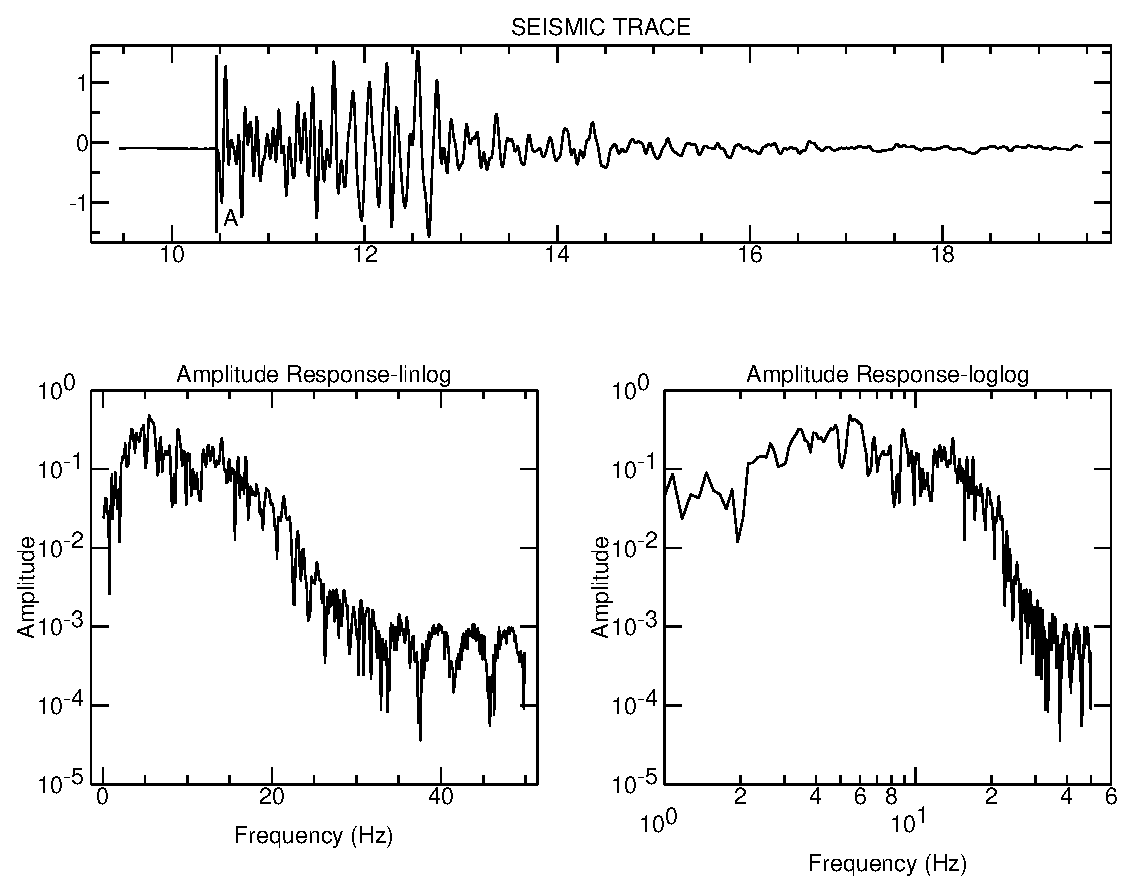
\includegraphics[width=14cm]{beginframe}
\caption{BEGINFRAME例子效果图}
\end{figure}

\SACTitle{相关命令}
ENDFRAME , XVPORT, YVPORT

\SACTitle{最近修订}
May 15, 1987 (Version 10.2)
